
\chapter{Language Design and Type System}
In this chapter, we'll design a subset of R with types and see how types and their operations could map to WASM generation.
\section{Design Goals}
Some reader at this point might be wondering why subset of R and why with types, why not just compile R to WASM. 
R is notoriously hard to compile to statically typed byte-code. A first reason is typing. 
\newline

\subsection{What makes R hard to compile}
\paragraph{Dynamic typing}
Let's take the following code.
\begin{lstlisting}
  x <- some_function()
\end{lstlisting}
WASM on the other hand is expecting variable \texttt{x} to have a type. There's 
\texttt{any} type in WASM. Maybe we can try mapping it to \texttt{anyref}. A reference to \texttt{any} element by the WASM GC proposal.
So now we have
\begin{lstlisting}
  (local $x anyref) // A tagged union can be also used.
\end{lstlisting}
Then, let's have a binary operation \texttt{x + y}, where \texttt{y} is also \texttt{anyref}.
Now we need to implement a generic function for plus operator that can potentially dispatch to all types of that function.
\begin{lstlisting}
  if x is int && y is int:
    add_int(x, y)
  if x is double && y is double:
    add_double(x, y)
  ...
\end{lstlisting}
This code will continue for every type and its combination. We'd have to also include promotion logic 
inside this code. Then x is int needs \texttt{try\_cast} as well. 
We'll need to do such generic function for every operation and functions. Some will be 
impossible to cover. This is essentially re-implementing the R interpreter.
Thus we fixate on R that's well-typed and the type is known or inferrable at compile time.

Moreover, we will see the same issue of dynamic dispatching when R variables change types.
\begin{lstlisting}
  x <- 5        # numeric
  x <- "hello"  # now a string
  x <- list()   # now a list
\end{lstlisting}
This bounds us to either writing generic functions or using wrappers like a tagged union, which will 
limit our performance and waste memory.

\paragraph{Changes in Runtime}
Change in built-in functions.
\begin{lstlisting}
  `+` <- function(x, y) x * y  # redefine addition!
\end{lstlisting}
This makes the job of compiler very hard.

\paragraph{Lazy Evaluation}
R uses lazy evaluation for function arguments; they're only evaluated when actually used:
\begin{lstlisting}
  f <- function(x, y) { if (x > 0) y else 0 }
  f(5, expensive_computation())  # expensive_computation() never runs!
\end{lstlisting}
This requires complex bookkeeping that's hard to optimize.

\paragraph{Reflection and Metaprogramming}
R code can inspect and modify itself at runtime:
\begin{lstlisting}
  x <- quote(a + b)  # capture unevaluated expression
  eval(x)            # evaluate it later
\end{lstlisting}

\paragraph{Non-Standard Evaluation (NSE)}
Many R functions evaluate arguments in non-standard ways:
\begin{lstlisting}
  subset(df, age > 30)  # 'age' isn't a variable, it's a column name!
\end{lstlisting}
This is extremely difficult to analyze statically.

In conclusion, all those issues outlined above, is not impossible to compile. However, they require
complex implementation and huge performance and memory trade-offs. For these, reasons it's important
for me to define the subset of R, which I can compile and limit the scope without losing R's main functionalities and purposes.

\section{Typed R-like Language}
This section presents the design of a statically-typed programming language inspired by R's syntax, which we refer to as the \textit{Typed R-like Language}. The language maintains R's characteristic features such as the left-assignment operator (\texttt{<-}), first-class functions, and vector-oriented programming, while introducing a static type system to enable ahead-of-time compilation to WebAssembly.
Below is table \ref{tab:r-typed-r-comparison0} comparing R and typed R in terms of features and design.

\begin{table}[h]
\centering
\begin{tabular}{|l|c|c|}
\hline
\textbf{Language Feature (Types)} & \textbf{R} & \textbf{Typed R} \\
% Basic Data Types
\hline
Integers & \checkmark & \checkmark \\
Doubles & \checkmark & \checkmark \\
Booleans & \checkmark & \checkmark \\
Strings & \checkmark & $\times$ \\
NULL/NA values & \checkmark & $\times$ \\
\hline

% Composite Data Types
Vectors & \checkmark & \checkmark \\
Matrices & \checkmark & $\times$ \\
Lists & \checkmark & $\times$ \\
Data frames & \checkmark & $\times$ \\
Arrays & \checkmark & $\times$ \\
\hline
\end{tabular}
\caption{Comparison of language features supported by R and Typed R}
\label{tab:r-typed-r-comparison0}
\end{table}

\begin{table}[h]
\centering
\begin{tabular}{|l|c|c|}
\hline
\textbf{Language Feature} & \textbf{R} & \textbf{Typed R} \\
% Basic Data Types
\hline

Static typing & $\times$ & \checkmark \\
First-class functions & \checkmark & \checkmark \\
Vector operations & \checkmark & \checkmark \\
Math operations & \checkmark & \checkmark \\
Control flow & \checkmark & \checkmark \\
Higher-order functions & \checkmark & \checkmark \\
Lexical scoping & \checkmark & \checkmark \\
Named arguments & \checkmark & \checkmark \\
Variable arguments (...) & \checkmark & \checkmark \\
\hline
Reflection & \checkmark & $\times$ \\
Runtime type changes & \checkmark & $\times$ \\
Non-standard evaluation (NSE) & \checkmark & $\times$ \\
Lazy evaluation & \checkmark & $\times$ \\
Copy-on-modify semantics & \checkmark & $\times$ \\
Garbage collection & \checkmark & \checkmark \\
Operator overloading & \checkmark & $\times$  \\
Attributes/metadata & \checkmark & $\times$  \\
Method dispatch (S3/S4/R6) & \checkmark & $\times$  \\

\hline
\end{tabular}
\caption{Comparison of language types supported by R and Typed R}
\label{tab:r-typed-r-comparison1}
\end{table}

The design philosophy emphasizes a familiar R-like syntax while ensuring type safety and efficient compilation to WebAssembly. Unlike dynamically-typed R, all type information is resolved at compile time, enabling optimized code generation and early error detection.

\section{Syntax}

The syntax of the Typed R-like Language closely follows R conventions with extensions for explicit type annotations. This section describes the core syntactic constructs.

\paragraph{Examples of Typed R}

\subparagraph{Variable Declaration and Assignment}

Variables are declared using the left-assignment operator with optional type annotations:

\begin{lstlisting}[language=R, caption={Variable assignment examples}]
# Simple assignment with type inference
x <- 10

# Assignment with explicit type annotation
y: int <- 20

# Vector assignment
vec <- c(1, 2, 3)
\end{lstlisting}

% \begin{lstlisting}[caption={Variable assignment in WAT}]
% (module
%   ;; Define array type for vectors
%   (type $vec_i32 (array (mut i32)))
  
%   (func $main
%     (local $x i32)
%     (local $y i32)
%     (local $vec (ref null $vec_i32))
    
%     ;; x <- 10
%     i32.const 10
%     local.set $x
    
%     ;; y: int <- 20
%     i32.const 20
%     local.set $y
    
%     ;; vec <- c(1, 2, 3)
%     i32.const 1
%     i32.const 2
%     i32.const 3
%     i32.const 3
%     array.new_fixed $vec_i32 3
%     local.set $vec
%   )
  
%   (start $main)
% )
% \end{lstlisting}

\subparagraph{Variable super-assignment}
The super-assignment operator \texttt{<<-} modifies variables in enclosing function scopes:

\begin{lstlisting}[language=R, caption={Super-assignment example}]
outer <- function() {
    x <- 0
    inner <- function() {
        x <<- 10  # Modifies x in outer scope
    }
    inner()
    return(x)  # Returns 10
}
\end{lstlisting}
\textit{In this case we see that it's identical to its R version}


\subparagraph{Function Definitions}

Functions are first-class values defined using the \texttt{function} keyword:

\begin{lstlisting}[language=R, caption={Function definition examples in typed R}]
# Simple function with type annotations
add <- function(a: int, b: int): int {
    return(a + b)
}

# Function returning a vector
create_vector <- function(): vector<double> {
    return(c(1.0, 2.0, 3.0))
}

# Higher-order function
apply_twice <- function(f: int -> int, x: int): int {
    return(f(f(x)))
}

\end{lstlisting}

% \begin{lstlisting}[caption={Function definition examples in WAT}]
% (module
%   ;; Define array type for double vectors
%   (type $vec_f64 (array (mut f64)))
  
%   ;; add <- function(a: int, b: int): int
%   (func $add (param $a i32) (param $b i32) (result i32)
%     local.get $a
%     local.get $b
%     i32.add
%   )
  
%   ;; create_vector <- function(): vector<double>
%   (func $create_vector (result (ref $vec_f64))
%     f64.const 1.0
%     f64.const 2.0
%     f64.const 3.0
%     i32.const 3
%     array.new_fixed $vec_f64 3
%   )
%   ;; apply_twice is not shown here.
  
% )
% \end{lstlisting}

\subparagraph{Conditional Statements}

The language supports \texttt{if-else} statements and expressions:

\begin{lstlisting}[language=R, caption={Conditional examples in typed R}]
# If statement
if (x > 0) {
    print(x)
}

# If-else statement
if (x > 0) {
    y <- 1
} else {
    y <- -1
}

# If expression (returns value)
result <- if (x > 0) { 1 } else { -1 }
\end{lstlisting}

% \begin{lstlisting}[caption={Conditional examples in WAT}]
% (module
%   ;; Import print function from host environment
%   (import "env" "print" (func $print (param i32)))
  
%   (func $main
%     (local $x i32)
%     (local $y i32)
    
%     ;; Set x to some value for demonstration
%     i32.const 5
%     local.set $x
    
%     ;; if (x > 0) { print(x) }
%     local.get $x
%     i32.const 0
%     i32.gt_s              ;; x > 0 (signed comparison)
%     if
%       local.get $x
%       call $print
%     end
    
%     ;; if (x > 0) { y <- 1 } else { y <- -1 }
%     local.get $x
%     i32.const 0
%     i32.gt_s              ;; x > 0
%     if
%       i32.const 1
%       local.set $y
%     else
%       i32.const -1
%       local.set $y
%     end
%   )
  
%   (start $main)
% )
% \end{lstlisting}

\subparagraph{Loops}

Two loop constructs are provided: \texttt{for} and \texttt{while}.

\begin{lstlisting}[language=R, caption={Loop examples}]
# For loop iterating over range
for (i in 1:10) {
    print(i)
}

# For loop iterating over vector
vec <- c(1, 2, 3, 4, 5)
for (x in vec) {
    print(x)
}

# While loop
i <- 1
sum <- 0
while (i <= 5) {
    sum <- sum + i
    i <- i + 1
}
\end{lstlisting}

% \begin{lstlisting}[caption={While loop examples in WAT}]
% (module
%   (func $main
%     (local $i i32)
%     (local $sum i32)
    
%     ;; i <- 1
%     i32.const 1
%     local.set $i
    
%     ;; sum <- 0
%     i32.const 0
%     local.set $sum
    
%     ;; while (i <= 5) { ... }
%     (block $break
%       (loop $continue
%         ;; Check condition: i <= 5
%         local.get $i
%         i32.const 5
%         i32.le_s            ;; i <= 5 (signed comparison)
%         i32.eqz             ;; negate: if NOT (i <= 5)
%         br_if $break        ;; break if condition is false
        
%         ;; sum <- sum + i
%         local.get $sum
%         local.get $i
%         i32.add
%         local.set $sum
        
%         ;; i <- i + 1
%         local.get $i
%         i32.const 1
%         i32.add
%         local.set $i
        
%         ;; Continue loop
%         br $continue
%       )
%     )
%   )
  
%   (start $main)
% )
% \end{lstlisting}


\subparagraph{Blocks and Tail Expressions}

Blocks consist of zero or more statements followed by an optional tail expression. The tail expression (final expression without semicolon) determines the block's value:

\begin{lstlisting}[language=R, caption={Block with tail expression}]
f <- function(x: int): int {
    y <- x * 2
    z <- y + 1
    z  # Tail expression - returned automatically
}
\end{lstlisting}

\subparagraph{Scoping and Closures}
\label{sec:scoping}

The language uses lexical scoping where:
\begin{itemize}
    \item Only functions create new scopes (blocks, if-statements, and loops do not)
    \item Functions can capture variables from enclosing function scopes
    \item Captured variables are implemented using closure environments in WebAssembly
    \item Super-assignment (\texttt{<<-}) searches enclosing function scopes to modify variables
\end{itemize}

Example demonstrating closure:
\begin{lstlisting}[language=R, caption={Closure example}]
make_counter <- function(start: int): () -> int {
    count <- start
    function(): int {
        count <<- count + 1
        return(count)
    }
}

counter <- make_counter(0)
print(counter())  # Prints 1
print(counter())  # Prints 2
\end{lstlisting}



\subsection{Abstract Grammar}

\begin{align*}
e ::= &\ x \quad \text{(variable)} \\
    &\mid n \mid d \mid \texttt{true} \mid \texttt{false} \quad \text{(literals)} \\
    &\mid \texttt{function}(p_1, \ldots, p_n): \tau\ \{\ e\ \} \quad \text{(function definition)} \\
    &\mid e_1(e_2, \ldots, e_n) \quad \text{(function call)} \\
    &\mid e_1(x_1{=}e_2, \ldots, x_n{=}e_n) \quad \text{(named argument call)} \\
    &\mid e_1 \oplus e_2 \quad \text{(binary operation)} \\
    &\mid \ominus e \quad \text{(unary operation)} \\
    &\mid \texttt{c}(e_1, \ldots, e_n) \quad \text{(vector construction)} \\
    &\mid e_1:e_2 \quad \text{(range sequence)} \\
    &\mid e_1[e_2] \quad \text{(vector indexing)} \\
    &\mid \texttt{if}\ e_1\ \{\ e_2\ \}\ \texttt{else}\ \{\ e_3\ \} \quad \text{(conditional)} \\
    &\mid \{\ e_1;\ \ldots;\ e_n\ \} \quad \text{(block)} \\
s ::= &\ x \gets e \quad \text{(assignment)} \\
    &\mid x: \tau \gets e \quad \text{(typed assignment)} \\
    &\mid x \ll\gets e \quad \text{(superassignment)} \\
    &\mid e \quad \text{(expression statement)} \\
    &\mid \texttt{return}(e) \quad \text{(return)} \\
    &\mid \texttt{for}\ (x\ \texttt{in}\ e)\ \{\ s\ \} \quad \text{(for loop)} \\
    &\mid \texttt{while}\ (e)\ \{\ s\ \} \quad \text{(while loop)} \\
p ::= &\ x: \tau \quad \text{(required parameter)} \\
    &\mid x: \tau = e \quad \text{(parameter with default)} \\
    &\mid \ldots \quad \text{(varargs)}
\end{align*}


\subsection{Lexical Elements}

The language uses the following lexical tokens:

\begin{itemize}
    \item \textbf{Keywords:} \texttt{function}, \texttt{if}, \texttt{else}, \texttt{for}, \texttt{in}, \texttt{while}, \texttt{return}
    \item \textbf{Type keywords:} \texttt{int}, \texttt{double}, \texttt{void}, \texttt{logical}, \texttt{vector}
    \item \textbf{Operators:}
    \begin{itemize}
        \item Assignment: \texttt{<-} (assignment), \texttt{<<-} (super-assignment)
        \item Arithmetic: \texttt{+}, \texttt{-}, \texttt{*}, \texttt{/}, \texttt{\%\%} (modulo)
        \item Comparison: \texttt{==}, \texttt{!=}, \texttt{<}, \texttt{<=}, \texttt{>}, \texttt{>=}
        \item Logical: \texttt{\&} (and), \texttt{|} (or), \texttt{!} (not)
        \item Range: \texttt{num1} \texttt{:} \texttt{num2} (sequence generation)
        \item Type annotation: \texttt{:} (in declaration context)
        \item Function arrow: \texttt{->} (in type signatures)
    \end{itemize}
    \item \textbf{Delimiters:} \texttt{(}, \texttt{)}, \texttt{\{}, \texttt{\}}, \texttt{[}, \texttt{]}, \texttt{,}
    \item \textbf{Literals:} Numeric literals, logical literals (\texttt{TRUE}, \texttt{FALSE})
    \item \textbf{Identifiers:} Alphanumeric sequences starting with a letter or underscore
    \item \textbf{Special:} \texttt{...} (varargs placeholder)
\end{itemize}

\section{Type System}
The type system ensures type safety through static analysis while supporting type inference to maintain concise syntax
and ease of development. 
Though it's important to note that there are many programs where type inference will fail to identify the type and our
compiler won't work due to lack of type information.

\begin{align*}
\tau ::= & \; num \mid \texttt{void} && \text{(base type)} \\
       | & \; \tau\texttt{[]} && \text{(vector type)} \\
       | & \; (\tau_1, \ldots, \tau_n) \to \tau && \text{(function type)} \\[0.5em]
num    ::= & \; \texttt{int} \mid \texttt{double} \mid \texttt{bool} && \text{(numeric types)}
\end{align*}

\paragraph{Primitive Types}

The language provides the following primitive types:

\begin{itemize}
    \item \texttt{int}: 32-bit signed integers (maps to WebAssembly \texttt{i32})
    \item \texttt{double}: 64-bit floating-point numbers (maps to WebAssembly \texttt{f64})
    \item \texttt{logical}: Boolean values (\texttt{TRUE} or \texttt{FALSE})
    \item \texttt{void}: Absence of value (used for functions with no return)
\end{itemize}
\paragraph{Logical}
Logicals will be represented as \texttt{int32} in WebAssembly, as it doesn't provide explicit type for logicals there.


\paragraph{Composite Types}

\subparagraph{Vector Types}

Vectors are homogeneous arrays parameterized by element type:

\begin{lstlisting}[language=R, caption={Vector type examples}]
# Vector of integers
v1: vector<int> <- c(1, 2, 3)

# Vector of doubles
v2: vector<double> <- c(1.5, 2.5, 3.5)

# Vector operations (component-wise)
v3: vector<double> <- v2 + c(1.0, 2.0, 3.0)
\end{lstlisting}

Vectors support component-wise arithmetic operations when both operands have compatible vector types.

\paragraph{Function Types}

Function types represent callable values with parameter and return types:

\begin{itemize}
    \item \texttt{int -> int}: Function taking an integer, returning an integer
    \item \texttt{int, int -> double}: Function taking two integers, returning a double
    \item \texttt{(int -> int) -> int}: Higher-order function taking a function as parameter
    \item \texttt{int, (int, int -> int) -> int}: Function taking an integer and a function
\end{itemize}

\subsection{Subtyping and Type Promotion}
Subtyping relation between logical, int, double and vectors are shown below \ref{fig:subtyping-hierarchy}.
For operations types are always implicitly casted to the wider types. From \texttt{logical $<:$ int $<:$ double}.
There's also vectors which are covariant to these types. For example \texttt{vector<int>} can be used in place of
\texttt{vector<double>}.
\begin{figure}[htbp]
\centering
\makebox[\textwidth][c]{%
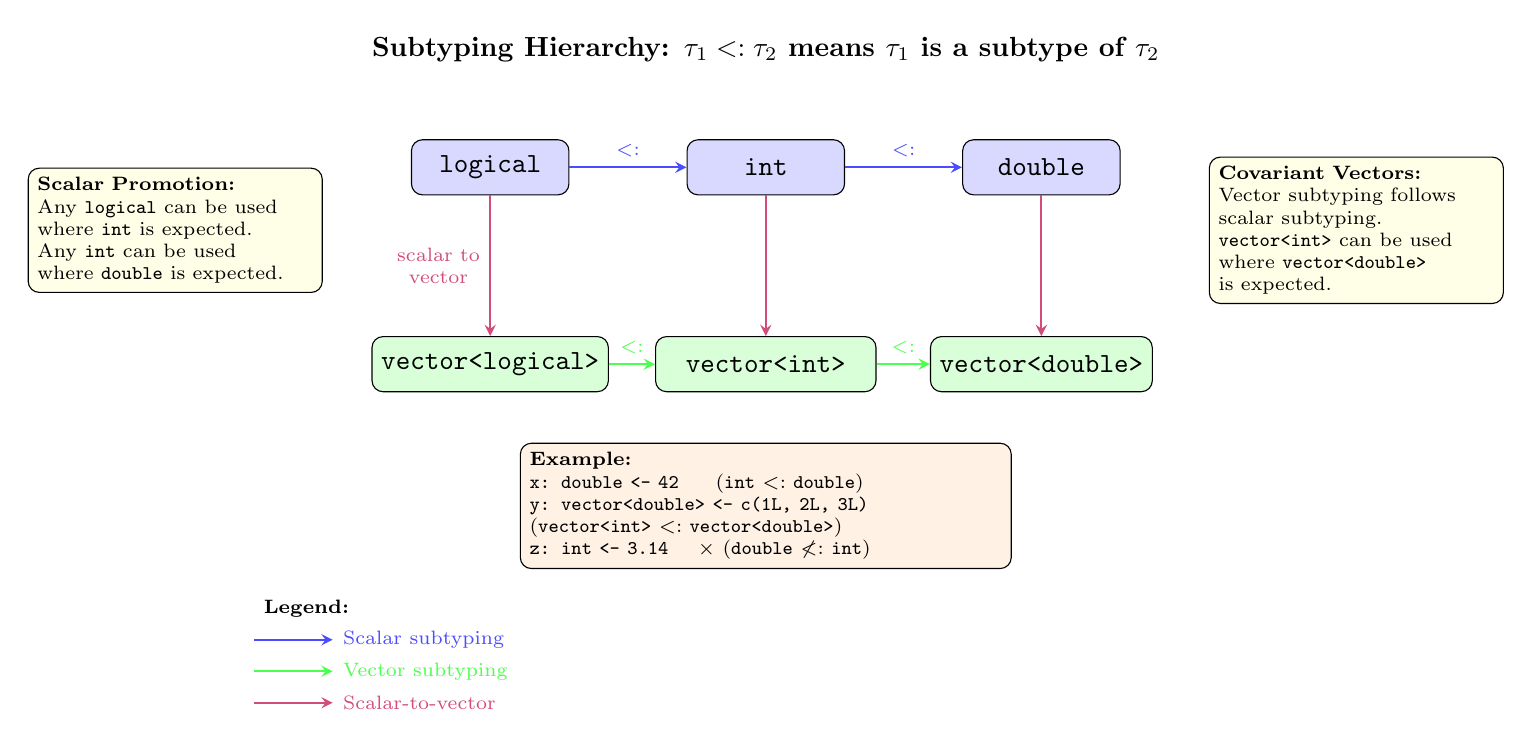
\begin{tikzpicture}[
    node distance=1.2cm,
    every node/.style={font=\small},
    scalarnode/.style={rectangle, draw, rounded corners, fill=blue!15, minimum width=2cm, minimum height=0.7cm, align=center, font=\ttfamily},
    vectornode/.style={rectangle, draw, rounded corners, fill=green!15, minimum width=2.8cm, minimum height=0.7cm, align=center, font=\ttfamily},
    subtype/.style={->, >=stealth, thick, blue!70},
    vecsubtype/.style={->, >=stealth, thick, green!70},
    crosssubtype/.style={->, >=stealth, thick, purple!70},
]

% Title
\node[font=\bfseries] at (0, 5.5) {Subtyping Hierarchy: $\tau_1 <: \tau_2$ means $\tau_1$ is a subtype of $\tau_2$};

% Scalar types (top row)
\node[scalarnode] (logical) at (-3.5, 4) {logical};
\node[scalarnode] (int) at (0, 4) {int};
\node[scalarnode] (double) at (3.5, 4) {double};

% Scalar subtyping arrows
\draw[subtype] (logical) -- node[above, font=\scriptsize] {$<:$} (int);
\draw[subtype] (int) -- node[above, font=\scriptsize] {$<:$} (double);

% Vector types (bottom row)
\node[vectornode] (veclogical) at (-3.5, 1.5) {vector<logical>};
\node[vectornode] (vecint) at (0, 1.5) {vector<int>};
\node[vectornode] (vecdouble) at (3.5, 1.5) {vector<double>};

% Vector subtyping arrows
\draw[vecsubtype] (veclogical) -- node[above, font=\scriptsize] {$<:$} (vecint);
\draw[vecsubtype] (vecint) -- node[above, font=\scriptsize] {$<:$} (vecdouble);

% Scalar to vector arrows (covariant)
\draw[crosssubtype] (logical) -- node[left, font=\scriptsize, align=center] {scalar to\\vector} (veclogical);
\draw[crosssubtype] (int) -- (vecint);
\draw[crosssubtype] (double) -- (vecdouble);

% Annotation boxes
\node[draw, rounded corners, fill=yellow!10, align=left, font=\scriptsize, text width=3.5cm] at (-7.5, 3.2) {
\textbf{Scalar Promotion:}\\
Any \texttt{logical} can be used\\
where \texttt{int} is expected.\\
Any \texttt{int} can be used\\
where \texttt{double} is expected.
};

\node[draw, rounded corners, fill=yellow!10, align=left, font=\scriptsize, text width=3.5cm] at (7.5, 3.2) {
\textbf{Covariant Vectors:}\\
Vector subtyping follows\\
scalar subtyping.\\
\texttt{vector<int>} can be used\\
where \texttt{vector<double>}\\
is expected.
};

% Example box
\node[draw, rounded corners, fill=orange!10, align=left, font=\scriptsize, text width=6cm] at (0, -0.3) {
\textbf{Example:}\\
\texttt{x: double <- 42} \quad $\checkmark$ (\texttt{int} $<:$ \texttt{double})\\
\texttt{y: vector<double> <- c(1L, 2L, 3L)} \quad $\checkmark$ (\texttt{vector<int>} $<:$ \texttt{vector<double>})\\
\texttt{z: int <- 3.14} \quad $\times$ (\texttt{double} $\not<:$ \texttt{int})
};

% Legend
\node[font=\scriptsize\bfseries, anchor=west] at (-6.5, -1.6) {Legend:};
\draw[subtype] (-6.5, -2) -- (-5.5, -2) node[anchor=west, font=\scriptsize] {Scalar subtyping};
\draw[vecsubtype] (-6.5, -2.4) -- (-5.5, -2.4) node[anchor=west, font=\scriptsize] {Vector subtyping};
\draw[crosssubtype] (-6.5, -2.8) -- (-5.5, -2.8) node[anchor=west, font=\scriptsize] {Scalar-to-vector};

\end{tikzpicture}%
}
\caption{Subtyping hierarchy showing scalar type promotion (\texttt{logical} $<:$ \texttt{int} $<:$ \texttt{double}) and covariant vector subtyping (\texttt{vector<logical>} $<:$ \texttt{vector<int>} $<:$ \texttt{vector<double>}). Scalar-to-vector conversions preserve the subtyping relationship, allowing implicit promotion in both scalar and vector contexts.}
\label{fig:subtyping-hierarchy}
\end{figure}

It's important to note, the language doesn't allow there's no user creatable subtyping. Currently,
we don't support S3 system, or any way to do OOP in Typed R.
\clearpage
\subsection{Type Checking}

The type checker performs bidirectional type inference\cite{bidirectional_typing}:

\begin{itemize}
    \item \textbf{Bottom-up inference:} Expression types are inferred from literal values and operator signatures
    \item \textbf{Top-down checking:} Function return types and variable annotations provide expected types
    \item \textbf{Unification:} Type constraints are solved to determine concrete types
\end{itemize}

Type annotations are required in the following contexts:
\begin{itemize}
    \item Function parameters
    \item Function return types (when not inferrable from return statements)
    \item Ambiguous variable declarations
\end{itemize}

Example: \texttt{3 + 2.5} evaluates as \texttt{3.0 + 2.5 = 5.5} after promoting \texttt{3} to \texttt{double}.

\begin{figure}[htbp]
\centering
\begin{tikzpicture}[
    node distance=0.4cm,
    every node/.style={font=\small},
    astnode/.style={rectangle, draw, minimum width=2.2cm, minimum height=0.7cm, align=center, fill=gray!5},
    typenode/.style={ellipse, draw, fill=blue!15, minimum width=1.8cm, minimum height=0.6cm, align=center, font=\small\ttfamily},
    constraint/.style={rectangle, rounded corners, draw, fill=orange!15, minimum width=3cm, minimum height=0.6cm, align=center, font=\footnotesize},
    arrow/.style={->, >=stealth, thick},
    typearrow/.style={->, >=stealth, dashed, blue, thick},
    checkarrow/.style={->, >=stealth, red!70, thick}
]

% Title
\node[font=\bfseries] at (0, 4.2) {Type Checking: \texttt{a: double <- 3.5}};

% AST Nodes
\node[astnode] (assign) at (0, 3) {Assignment\\$\texttt{a} \leftarrow$};
\node[astnode] (decl) at (-3, 1.8) {Variable\\Declaration: \texttt{a}};
\node[astnode] (literal) at (3, 1.8) {Literal\\Expression: \texttt{3.5}};

% Type annotations
\node[typenode] (decltype) at (-3, 0.6) {double};
\node[typenode] (littype) at (3, 0.6) {double};

% Connections
\draw[arrow] (assign) -- (decl);
\draw[arrow] (assign) -- (literal);

% Type inference (bottom-up)
\draw[typearrow] (literal) -- node[right, font=\scriptsize, text=blue!70] {infer} (littype);

% Type annotation (top-down)
\draw[typearrow] (decl) -- node[left, font=\scriptsize, text=blue!70] {annotate} (decltype);

% Unification
\node[constraint] (unify) at (0, 0.6) {Unification Check};
\draw[checkarrow] (decltype) -- (unify);
\draw[checkarrow] (littype) -- (unify);

% Success indicator
\node[constraint, fill=green!20] (success) at (0, -0.4) { Type Check Passes: \texttt{double = double}};
\draw[arrow, green!70!black, thick] (unify) -- (success);

% Step-by-step annotation boxes
\node[anchor=west, font=\scriptsize, align=left, draw, rounded corners, fill=yellow!10, minimum width=4.5cm] at (5, 3) {
\textbf{Step 1: Top-down}\\
Parse annotation \texttt{a: double}\\
Expected type: \texttt{double}
};

\node[anchor=west, font=\scriptsize, align=left, draw, rounded corners, fill=yellow!10, minimum width=4.5cm] at (5, 1.5) {
\textbf{Step 2: Bottom-up}\\
Infer literal \texttt{3.5}\\
Inferred type: \texttt{double}
};

\node[anchor=west, font=\scriptsize, align=left, draw, rounded corners, fill=yellow!10, minimum width=4.5cm] at (5, 0) {
\textbf{Step 3: Unify}\\
Check: \texttt{double} $\stackrel{?}{=}$ \texttt{double}\\
Result: \textcolor{green!70!black}{\textbf{Success!}}
};

% Legend
\node[font=\scriptsize\bfseries, anchor=west] at (-5, -1.3) {Legend:};
\draw[arrow] (-5, -1.7) -- (-4.2, -1.7) node[anchor=west, font=\scriptsize] {AST structure};
\draw[typearrow] (-5, -2.1) -- (-4.2, -2.1) node[anchor=west, font=\scriptsize] {Type flow};
\draw[checkarrow] (-5, -2.5) -- (-4.2, -2.5) node[anchor=west, font=\scriptsize] {Unification};

\end{tikzpicture}
\caption{Bidirectional type checking for variable assignment. The type annotation \texttt{double} provides the expected type (top-down), while the literal \texttt{3.5} has its type inferred as \texttt{double} (bottom-up). The unification step verifies that both types match, allowing the assignment to proceed.}
\label{fig:type-checking-simple}
\end{figure}

\subsection{Typing Rules}

This section formalizes the type system using inference rules. We use \textbf{typing judgments} of the form:
\[
\Gamma \vdash e : \tau
\]
This is read as: ``under typing context $\Gamma$, expression $e$ has type $\tau$.'' The typing context $\Gamma$ maps variable names to their types. The rules are presented in natural deduction style, where premises appear above the horizontal line and the conclusion below. A rule with no premises (nothing above the line) is an \textbf{axiom}---it holds unconditionally.

Our type system follows standard approaches from programming language theory~\cite{types_and_pl}, extended with subtyping for numeric promotion and vector operations.

\paragraph{Typing Contexts}

A \textbf{typing context} (or type environment) is a finite mapping from variable names to types:
\[
\Gamma ::= \emptyset \mid \Gamma, x:\tau
\]

The empty context $\emptyset$ contains no bindings. The notation $\Gamma, x:\tau$ extends context $\Gamma$ with a new binding of variable $x$ to type $\tau$. We write $x:\tau \in \Gamma$ to indicate that $\Gamma$ contains the binding $x:\tau$.

\paragraph{Subtyping}

Subtyping defines when one type can be safely used where another is expected. We write $\tau_1 <: \tau_2$ to mean ``$\tau_1$ is a subtype of $\tau_2$'' (equivalently, $\tau_1$ can be used wherever $\tau_2$ is expected).

\paragraph{Reflexivity and Base Cases}
Every type is a subtype of itself, and we define the numeric promotion hierarchy:

\begin{mathpar}
\inferrule*[right=S-Refl]
    {\ }
    {\tau <: \tau}

\and

\inferrule*[right=S-LogicalInt]
    {\ }
    {\texttt{logical} <: \texttt{int}}

\and

\inferrule*[right=S-IntDouble]
    {\ }
    {\texttt{int} <: \texttt{double}}
\end{mathpar}

\textbf{Explanation:} \textsc{S-Refl} states that any type is a subtype of itself (reflexivity). \textsc{S-LogicalInt} allows logical values (represented as 0 or 1) to be used as integers. \textsc{S-IntDouble} allows integers to be promoted to doubles, enabling mixed arithmetic like \texttt{3 + 2.5}.

\paragraph{Transitivity}
Subtyping is transitive, allowing chains like $\texttt{logical} <: \texttt{int} <: \texttt{double}$:

\begin{mathpar}
\inferrule*[right=S-Trans]
    {\tau_1 <: \tau_2 \\ \tau_2 <: \tau_3}
    {\tau_1 <: \tau_3}
\end{mathpar}

\textbf{Explanation:} If $\tau_1$ can be used as $\tau_2$, and $\tau_2$ can be used as $\tau_3$, then $\tau_1$ can be used as $\tau_3$. This gives us $\texttt{logical} <: \texttt{double}$ automatically.

\paragraph{Vector Covariance}
Vectors are \textbf{covariant} in their element type:

\begin{mathpar}
\inferrule*[right=S-Vector]
    {\tau_1 <: \tau_2}
    {\texttt{vector}\langle\tau_1\rangle <: \texttt{vector}\langle\tau_2\rangle}
\end{mathpar}

\textbf{Explanation:} If element type $\tau_1$ is a subtype of $\tau_2$, then a vector of $\tau_1$ can be used where a vector of $\tau_2$ is expected. For example, \texttt{vector<int>} $<:$ \texttt{vector<double>}, so an integer vector can be passed to a function expecting a double vector.

\paragraph{Subsumption}
The \textbf{subsumption rule} connects subtyping to the type system, allowing implicit type promotion:

\begin{mathpar}
\inferrule*[right=T-Sub]
    {\Gamma \vdash e : \tau_1 \\ \tau_1 <: \tau_2}
    {\Gamma \vdash e : \tau_2}
\end{mathpar}

\textbf{Explanation:} If expression $e$ has type $\tau_1$ and $\tau_1$ is a subtype of $\tau_2$, then $e$ can also be given type $\tau_2$. This rule enables all implicit conversions in the language. For example, if \texttt{x} has type \texttt{int}, we can use it where \texttt{double} is expected.

\paragraph{Literals and Variables}

These rules assign types to the basic building blocks of expressions.

\begin{mathpar}
\inferrule*[right=T-Int]
    {n \in \mathbb{Z}}
    {\Gamma \vdash n : \texttt{int}}

\and

\inferrule*[right=T-Double]
    {d \in \mathbb{R}}
    {\Gamma \vdash d : \texttt{double}}

\and

\inferrule*[right=T-Bool]
    {b \in \{\texttt{TRUE}, \texttt{FALSE}\}}
    {\Gamma \vdash b : \texttt{logical}}

\and

\inferrule*[right=T-Var]
    {x:\tau \in \Gamma}
    {\Gamma \vdash x : \tau}
\end{mathpar}

\textbf{Explanation:}
\begin{itemize}
    \item \textsc{T-Int}: Integer literals like \texttt{42} or \texttt{-7} have type \texttt{int}.
    \item \textsc{T-Double}: Floating-point literals like \texttt{3.14} have type \texttt{double}.
    \item \textsc{T-Bool}: The literals \texttt{TRUE} and \texttt{FALSE} have type \texttt{logical}.
    \item \textsc{T-Var}: A variable $x$ has whatever type the context $\Gamma$ says it has. This rule performs a lookup in the typing environment.
\end{itemize}

\paragraph{Arithmetic Operators}

Arithmetic operators (\texttt{+}, \texttt{-}, \texttt{*}, \texttt{/}, \texttt{\%\%}) follow the same typing pattern. We show rules for addition; other operators are analogous.

\begin{mathpar}
\inferrule*[right=T-AddInt]
    {\Gamma \vdash e_1 : \texttt{int} \\ \Gamma \vdash e_2 : \texttt{int}}
    {\Gamma \vdash e_1 + e_2 : \texttt{int}}

\and

\inferrule*[right=T-AddDouble]
    {\Gamma \vdash e_1 : \texttt{double} \\ \Gamma \vdash e_2 : \texttt{double}}
    {\Gamma \vdash e_1 + e_2 : \texttt{double}}
\end{mathpar}

\textbf{Explanation:} When both operands have the same numeric type, the result has that type. Note that mixed-type arithmetic like \texttt{3 + 2.5} is handled by first applying subsumption (\textsc{T-Sub}) to promote \texttt{3} from \texttt{int} to \texttt{double}, then applying \textsc{T-AddDouble}.

\paragraph{Comparison Operators}

Comparison operators (\texttt{==}, \texttt{!=}, \texttt{<}, \texttt{<=}, \texttt{>}, \texttt{>=}) compare values and produce logical results:

\begin{mathpar}
\inferrule*[right=T-Compare]
    {\Gamma \vdash e_1 : \tau \\ \Gamma \vdash e_2 : \tau \\ \tau \in \{\texttt{int}, \texttt{double}, \texttt{logical}\}}
    {\Gamma \vdash e_1 \odot e_2 : \texttt{logical}}
\end{mathpar}

where $\odot \in \{\texttt{==}, \texttt{!=}, \texttt{<}, \texttt{<=}, \texttt{>}, \texttt{>=}\}$.

\textbf{Explanation:} Comparisons require both operands to have the same type (after potential promotion via subsumption) and always produce a \texttt{logical} result. For example, \texttt{3 < 5} produces \texttt{TRUE}.

\paragraph{Logical Operators}

Logical operators work on boolean values:

\begin{mathpar}
\inferrule*[right=T-And]
    {\Gamma \vdash e_1 : \texttt{logical} \\ \Gamma \vdash e_2 : \texttt{logical}}
    {\Gamma \vdash e_1\ \texttt{\&}\ e_2 : \texttt{logical}}

\and

\inferrule*[right=T-Or]
    {\Gamma \vdash e_1 : \texttt{logical} \\ \Gamma \vdash e_2 : \texttt{logical}}
    {\Gamma \vdash e_1\ \texttt{|}\ e_2 : \texttt{logical}}

\and

\inferrule*[right=T-Not]
    {\Gamma \vdash e : \texttt{logical}}
    {\Gamma \vdash \texttt{!}e : \texttt{logical}}
\end{mathpar}

\textbf{Explanation:} Logical AND (\texttt{\&}), OR (\texttt{|}), and NOT (\texttt{!}) require logical operands and produce logical results.

\paragraph{Vector Construction}
The \texttt{c()} function creates vectors from elements:

\begin{mathpar}
\inferrule*[right=T-Vector]
    {\Gamma \vdash e_1 : \tau \\ \Gamma \vdash e_2 : \tau \\ \cdots \\ \Gamma \vdash e_n : \tau}
    {\Gamma \vdash \texttt{c}(e_1, e_2, \ldots, e_n) : \texttt{vector}\langle\tau\rangle}
\end{mathpar}

\textbf{Explanation:} All elements must have the same type $\tau$ (after promotion). The result is a vector parameterized by that element type. For example, \texttt{c(1, 2, 3)} has type \texttt{vector<double>}.

\paragraph{Range Construction}
The colon operator creates sequences:

\begin{mathpar}
\inferrule*[right=T-Range]
    {\Gamma \vdash e_1 : \tau_1 \\ \Gamma \vdash e_2 : \tau_2 \\ \tau_1, \tau_2 \in \{\texttt{int}, \texttt{double}\}}
    {\Gamma \vdash e_1\texttt{:}e_2 : \texttt{vector}\langle\tau_1 \sqcup \tau_2\rangle}
\end{mathpar}

where $\tau_1 \sqcup \tau_2$ denotes the \textbf{least upper bound} (join) of the two types under the subtyping relation:
\[
\texttt{int} \sqcup \texttt{int} = \texttt{int} \qquad
\texttt{double} \sqcup \texttt{double} = \texttt{double} \qquad
\texttt{int} \sqcup \texttt{double} = \texttt{double}
\]

\textbf{Explanation:} The range \texttt{1:5} creates the sequence from 1 to 5. The element type is the wider of the two bound types: \texttt{1L:5L} produces \texttt{vector<int>}, while \texttt{1:5} or \texttt{1L:5.0} produces \texttt{vector<double>}.

\paragraph{Vector Indexing}
Elements are accessed using bracket notation:

\begin{mathpar}
\inferrule*[right=T-Index]
    {\Gamma \vdash e_1 : \texttt{vector}\langle\tau\rangle \\ \Gamma \vdash e_2 : \tau' \\ \tau' \in \{\texttt{int}, \texttt{double}\}}
    {\Gamma \vdash e_1[e_2] : \tau}
\end{mathpar}

\textbf{Explanation:} Indexing a vector of type \texttt{vector<$\tau$>} produces a value of type $\tau$. The index can be an integer or double; doubles are truncated to integers at runtime. Following R convention, indexing is 1-based.

\paragraph{Vector Arithmetic}
Binary operators extend component-wise to vectors:

\begin{mathpar}
\inferrule*[right=T-VecBinOp]
    {\Gamma \vdash e_1 : \texttt{vector}\langle\tau\rangle \\ \Gamma \vdash e_2 : \texttt{vector}\langle\tau\rangle \\ \tau \in \{\texttt{int}, \texttt{double}\}}
    {\Gamma \vdash e_1 \oplus e_2 : \texttt{vector}\langle\tau\rangle}
\end{mathpar}

where $\oplus \in \{+, -, *, /, \texttt{\%\%}\}$.

\textbf{Explanation:} When both operands are vectors of the same numeric type, the operation applies element-wise. For example, \texttt{c(1,2) + c(3,4)} produces \texttt{c(4,6)}.

\paragraph{Scalar-Vector Operations}
Scalars broadcast to match vector length:

\begin{mathpar}
\inferrule*[right=T-ScalarVec]
    {\Gamma \vdash e_1 : \tau \\ \Gamma \vdash e_2 : \texttt{vector}\langle\tau\rangle \\ \tau \in \{\texttt{int}, \texttt{double}\}}
    {\Gamma \vdash e_1 \oplus e_2 : \texttt{vector}\langle\tau\rangle}
\end{mathpar}

\textbf{Explanation:} A scalar is implicitly replicated to match the vector length. For example, \texttt{2 * c(1,2,3)} produces \texttt{c(2,4,6)}. The symmetric case (vector $\oplus$ scalar) follows analogously.

\subsubsection{Functions}

\paragraph{Function Definition}
Functions are first-class values with explicit parameter and return types:

\begin{mathpar}
\inferrule*[right=T-Func]
    {\Gamma, x_1:\tau_1, \ldots, x_n:\tau_n \vdash e : \tau}
    {\Gamma \vdash \texttt{function}(x_1:\tau_1, \ldots, x_n:\tau_n):\tau\ \{\ e\ \} : (\tau_1, \ldots, \tau_n) \to \tau}
\end{mathpar}

\textbf{Explanation:} To type-check a function, we extend the context with the parameter bindings and check that the body $e$ has the declared return type $\tau$. The function itself has a \textbf{function type} $(\tau_1, \ldots, \tau_n) \to \tau$ indicating it takes $n$ arguments of types $\tau_1, \ldots, \tau_n$ and returns type $\tau$.

\paragraph{Function Application}
Function calls check argument types against parameter types:

\begin{mathpar}
\inferrule*[right=T-App]
    {\Gamma \vdash e_0 : (\tau_1, \ldots, \tau_n) \to \tau \\ \Gamma \vdash e_1 : \tau_1 \\ \cdots \\ \Gamma \vdash e_n : \tau_n}
    {\Gamma \vdash e_0(e_1, \ldots, e_n) : \tau}
\end{mathpar}

\textbf{Explanation:} To call a function, the callee $e_0$ must have a function type, and each argument must match the corresponding parameter type (or be promotable via subsumption). The result has the function's return type.

\paragraph{Conditional Expressions}
If-else expressions require matching branch types:

\begin{mathpar}
\inferrule*[right=T-If]
    {\Gamma \vdash e_1 : \texttt{logical} \\ \Gamma \vdash e_2 : \tau \\ \Gamma \vdash e_3 : \tau}
    {\Gamma \vdash \texttt{if}\ (e_1)\ \{e_2\}\ \texttt{else}\ \{e_3\} : \tau}
\end{mathpar}

\textbf{Explanation:} The condition must be logical. Both branches must have the same type $\tau$, which becomes the type of the entire expression. This enables using if-else as an expression: \texttt{x <- if (cond) \{ 1 \} else \{ 2 \}}.

\paragraph{Assignment}
Assignment binds a value to a variable, extending the context:

\begin{mathpar}
\inferrule*[right=T-Assign]
    {\Gamma \vdash e : \tau}
    {\Gamma \vdash (x \gets e) : \tau \dashv \Gamma, x:\tau}
\end{mathpar}

\textbf{Explanation:} We use $\dashv \Gamma'$ to indicate the \textbf{output context} after the statement. Assignment evaluates $e$, binds the result to $x$, and produces an updated context where $x$ has type $\tau$. The assignment itself also has type $\tau$ (assignments are expressions in R).

\paragraph{Super-Assignment}
Super-assignment modifies a variable in an enclosing scope:

\begin{mathpar}
\inferrule*[right=T-SuperAssign]
    {x:\tau \in \Gamma_{outer} \\ \Gamma \vdash e : \tau'}
    {\Gamma \vdash (x \ll\gets e) : \tau'}
\end{mathpar}

where $\tau' <: \tau$ (the assigned value must be compatible with the existing binding).

\textbf{Explanation:} Super-assignment requires that $x$ already exists in some enclosing function scope ($\Gamma_{outer}$). The expression type must be compatible with the existing variable's type.

\paragraph{Blocks}
A block is a sequence of statements with an optional tail expression:

\begin{mathpar}
\inferrule*[right=T-Block]
    {\Gamma \vdash s_1 : \tau_1 \dashv \Gamma_1 \\ \Gamma_1 \vdash s_2 : \tau_2 \dashv \Gamma_2 \\ \cdots \\ \Gamma_{n-1} \vdash e : \tau}
    {\Gamma \vdash \{s_1; s_2; \ldots; e\} : \tau}
\end{mathpar}

\textbf{Explanation:} Statements are checked in sequence, with each statement potentially extending the context for subsequent statements. The block's type is determined by its final expression (the tail expression).

\paragraph{Return Statement}

\begin{mathpar}
\inferrule*[right=T-Return]
    {\Gamma \vdash e : \tau}
    {\Gamma \vdash \texttt{return}(e) : \tau}
\end{mathpar}

\textbf{Explanation:} A return statement has the type of its argument. The type checker verifies that this matches the declared return type of the enclosing function.


\section{Evaluation Model}

This section describes the key runtime behaviors that affect how programs execute and how the compiler generates code.

\paragraph{Evaluation Order and Type Promotion}

Expressions are evaluated left-to-right. When operands have different numeric types, the narrower type is promoted to the wider type before the operation:
\begin{itemize}
    \item \texttt{logical} $\to$ \texttt{int}: \texttt{TRUE} becomes \texttt{1}, \texttt{FALSE} becomes \texttt{0}
    \item \texttt{int} $\to$ \texttt{double}: integers are converted to floating-point
\end{itemize}

For example, \texttt{TRUE + 2.5} evaluates as \texttt{1.0 + 2.5 = 3.5} (logical $\to$ int $\to$ double).

\paragraph{Vector Operations}

Vector operations apply element-wise. When vectors have different element types, promotion occurs element-by-element:
\[
\texttt{c}(v_1, \ldots, v_n) \oplus \texttt{c}(w_1, \ldots, w_n) = \texttt{c}(v_1 \oplus w_1, \ldots, v_n \oplus w_n)
\]
When the length of the vector differs, we use recycling like in R. Essentially the vector of lower length
is permutated until it has same or more length as the vector with higher length and operation is executed. For R, when the length
of one vector is not divisible by the other, meaning the permutated vector will have additional elements, that won't be included in the operation,
standard R environment shows a warning message. However, we don't have warning message in our compiler yet, it won't be provided.

\paragraph{Scalar Broadcasting}
When a scalar and vector are combined, the scalar is implicitly broadcast (replicated) to match the vector length:
\[
s \oplus \texttt{c}(v_1, \ldots, v_n) = \texttt{c}(s \oplus v_1, \ldots, s \oplus v_n)
\]
For example, \texttt{2 * c(1, 2, 3)} produces \texttt{c(2, 4, 6)}.

\paragraph{Function Evaluation and Closures}

Functions in the typed R-like language are \textbf{closures}: they capture the environment in which they are defined. When a function is called:
\begin{enumerate}
    \item The callee expression is evaluated to obtain a closure (function code + captured environment)
    \item Arguments are evaluated left-to-right in the caller's environment
    \item A new environment is created, extending the closure's captured environment with parameter bindings
    \item The function body is evaluated in this new environment
\end{enumerate}

It'll be discussed more in details in compiler and runtime environment in Chapter~\ref{chapter:compiler}.

\subsection{Built-in Functions}

The language provides the following built-in functions:

\begin{table}[h]
\centering
\begin{tabular}{|l|l|l|}
\hline
\textbf{Function} & \textbf{Type} & \textbf{Description} \\
\hline
\texttt{c(e1, ..., en)} & $(\tau, \ldots, \tau) \to \texttt{vector}\langle\tau\rangle$ & Creates vector from elements \\
\texttt{print(e)} & $\tau \to \texttt{void}$ & Outputs value to stdout \\
\texttt{length(v)} & $\texttt{vector}\langle\tau\rangle \to \texttt{int}$ & Returns vector length \\
\texttt{sum(v)} & $\texttt{vector}\langle\tau\rangle \to \tau$ & Sums numeric vector \\
\hline
\end{tabular}
\caption{Built-in functions and their types}
\label{tab:builtins}
\end{table}
